\section{Tauri}
\label{sec:tauri}
Tauri was first released at \displaydate{dateTauriRelease}~\cite{tauriRelease} and downloaded approx. $58\,000$ times\footnote{According to \url{https://npm-stat.com/charts.html?package=tauri&from=2019-12-31&to=2022-08-12}}.
It resulted as discontent of Electron from the Tauri developers especially in case of resource consumption and security due to uncontrollable dependencies~\cite{tauri}.
They criticized the enormous resource consumption even of the simplest applications as well as the fact that Electron does not have control over their dependencies.
If Chromium encounters a zero-day-exploit and releases a patch, Electron has to include this patch and also release a newer version.
This results in requiring users of an Electron-based application, to update their Electron Version to close this security issue.
This timespan between first fix of Chromium and the users update of the application poses a high vulnerability against potential attackers.
In this regard, the developers also criticized the power of the privileges Electron applications require, allowing attackers to have access to the entire hard drive of the user for example~\cite{tauri}.
Like Electron, Tauri experienced increasing attention, mentioning that the first stable version has been released in 2022.
This attention can also be expressed numerically in terms of usage, forks or contributions of developers, as in Chapter~\ref{sec:electron}.
Table~\ref{tab:tauri:statistics} is showing these numbers based on GitHub Statistics~\cite{GithubTauri}: \\ \\
\begin{table}[h]
    \begin{tabular} {| c | c | c | c | c |}
        Stars      & Forks     & Watching & Used by    & Contributors \\ \hline
        $48\,200$ & $1\,200$ & $403$ & $3\,200$ & $182$
    \end{tabular}
    \caption{\label{tab:tauri:statistics} GitHub Statistics of the Tauri repository}
\end{table}\\ \\ \newpage
In contrast to Electron, Tauri uses the self developed core called Tauri, written in Rust in combination with \ac{WRY} that serves as the rendering library.


\subsection{Architecture}
\label{subsec:tauri:architecture}
The architecture of Tauri is quite similar to Electrons multiprocess model.
Tauri also relies on a main process, called \textbf{core} process and multiple rendering processes, called \textbf{webview} for performance as well as security reasons.
\figref{fig:tauri:model} shows the basic architecture of Tauris multiprocess model, whereas each \texttt{webview} process is managed by the \texttt{core} process.
\begin{figure}[ht]
    \centering
    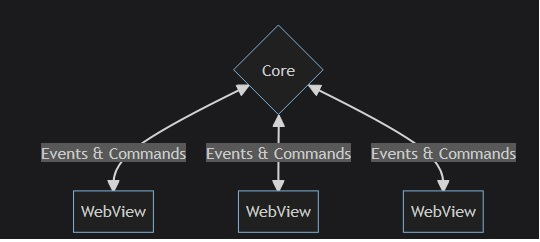
\includegraphics[width=0.4\textwidth]{images/TauriArchitecture}
    \caption{Multi-process Model Tauri from~\cite{tauri}}
    \label{fig:tauri:model}
\end{figure}

\begin{description}
    \item[\textbf{Core}:] \hfill \\ This is the main entry point of the application and the only place where full access to the operating system is provided.
    The \texttt{core} process uses these privileges to create and manage the windows of the application.
    It is also the only point, where the communication between processes is going through, allowing the \texttt{core} process to manipulate or observe \ac{IPC} messages.
    Unlike Electron, \texttt{webview} processes are not able to communicate directly between each other, increasing the security, since each message has to pass the \texttt{core} process and
    can be discarded if suspicious or unwanted calls are made.
    Additionally, the \texttt{core} process is responsible for global scoped cases such as database access, managing application or \ac{OS}-specific settings affecting the windows.
    Summarized it serves as a centralized management and control point, where the application as itself is maintained and sensitive data is kept to be hidden from the \texttt{webview} processes~\cite{tauri}.


    \item[\textbf{WebView}:] \hfill \\ A \texttt{webview} process renders the \ac{HTML} content of an application using the WebView libraries of the current \ac{OS}.
    Since this library is not included into the final executable but linked at runtime, its appearance differs depending on the \ac{OS} the application is running at.
    This reduces the size of the executable, since the part where the actual rendering takes places is shifted from the application to the \ac{OS}, but also forces
    developers to consider and keep in mind the different \ac{OS}s~\cite{tauri}.

\end{description}
 \newpage
\subsubsection{Inter Process Communication}
For communication between different processes Tauri also uses Inter Process Communication similar to Electron.
\begin{figure}[ht]
    \centering
    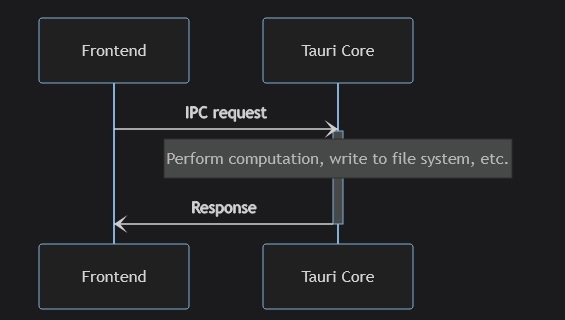
\includegraphics[width=0.4\textwidth]{images/TauriIPC}
    \caption{IPC of Tauri~\cite[Figure 1--3]{tauri}}
    \label{fig:tauri:ipc}
\end{figure}
In contrast, Tauri forces developers from the beginning to use the \ac{AMP} paradigm, whereas Electron released this feature at version 14 and only recommends it.
The main advantage of \ac{AMP} is that direct function access is denied and thus all communication has to pass the \texttt{core} process.
Since it is able to observe the content of messages, it can decide which message will be forwarded and which will be blocked, for instance malicious requests.
Communication can either be unidirectional using events or bidirectional using commands, which are both \ac{IPC} messages.
Events can be emitted by both \texttt{core} and \texttt{webview} processes to inform the event recipient but without any response.
In contrast commands can only be emitted by the \texttt{webview} processes to invoke functions that require access to the operating system as shown in \figref{fig:tauri:ipc}.
The \texttt{core} process itself is not able to emit commands to the frontend, preventing potential malicious code segments inside the \texttt{core} process affecting the \texttt{webview} processes~\cite{tauri}.

\subsubsection{Context Isolation}
In contrast to Electron, Tauri uses different patterns for isolating communication between the \texttt{webview} processes and the \texttt{core} process and potential critical \ac{API} calls.
They are called Brownfield and Isolation Pattern, whereas the default pattern that can be configured inside the \texttt{tauri.conf.json} is the Brownfield pattern.
\begin{description}
    \item[\textbf{Brownfield Pattern}:] \hfill \\
    The Brownfield pattern can be seen as a design pattern to ensure interoperability between new implemented and existing software.
    This pattern does not categorize software as legacy software but as current state of the art.
    Software developed following this pattern tries to coexist and to consider existing software as much as possible.
    This requires a deep knowledge of the existing software and can also result in re-developing significant parts of the existing software when trying to enhance new features.
    Tauri uses this pattern as standard and explains that it tries to be as compatible as possible.
    But unfortunately Tauri does not explain in detail how they are implementing this pattern and how this helps to avoid malicious frontend calls to the Tauri core~\cite{tauri}. \\
    \item[\textbf{Isolation Pattern}:] \hfill \\
    The Isolation Pattern can be seen as an interposed instance between the \ac{IPC} handler and the processes.
    This instance is providing a sandbox, called Isolation application, which is trusted and secure JavaScript code embedded into an \texttt{<iframe>}.
    The \ac{IPC} handler passes its message to the Isolation application, where it is executed and may be modified or verified.
    After that it will be encrypted, passed back to the \ac{IPC} handler and forwarded to the \texttt{core} process, where it will be handled as normal~\cite{tauri}.


\end{description}

\begin{figure}[ht]
    \centering
    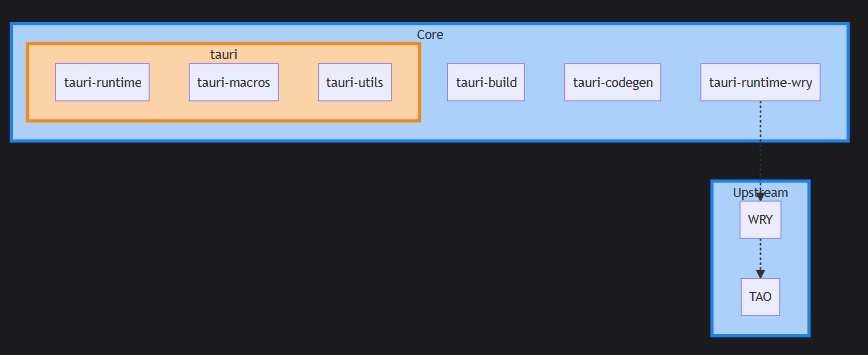
\includegraphics[width=0.4\textwidth]{images/TauriCore}
    \caption{Core Ecosystem from~\cite{tauri}}
    \label{fig:tauri:core}
\end{figure}
As can be seen in \figref{fig:tauri:core}, Tauri splits its framework into two main components.
The Core, containing several modules providing \ac{API} access, utilities and the runtime, can be seen as the backend part of the framework.
The Upstream component, serving as the frontend part contains the two self-developed Rust crates \ac{WRY} and TAO, proper name, which are providing libraries for creating browser windows and rendering the WebView and its content.
%Same as described for Tauri.Ref to introduction\ref{subsec:electron:arch}

\subsection{Frontend}
\label{subsec:tauri:frontend}
Tauris frontend relies on its own implementation of WebView instead of the entire Chromium content module for rendering \ac{HTML} content.
This makes it much smaller than Electron applications since their libraries \ac{WRY} and TAO are using the exising web engines of the three major \ac{OS} Linux, macOS and Windows instead of shipping an entire browser.
\begin{description}
    \item[\textbf{TAO}:] \hfill \\
    TAO is a cross-platform library written in Rust and used for creating and managing application windows.
    It was forked from the Rust crate \texttt{winit}, since the developers wanted to enhance more desktop features than the original crate, for instance menu bars or a system tray.
    The library ships with an entire event loop that can be emitted by windows, for example resizing or key interactions and is included at the second frontend library \ac{WRY}~\cite{TAO}\@.
    \item[\textbf{\ac{WRY}}:] \hfill \\
    \ac{WRY} is the main library of Tauri applications, based on the webview library~\cite{githubWebview} and responsible for rendering the content of the \ac{OS}-specific webview.
    It acts as an interface between the Tauri core with its low level webview drivers and the webview technology of the current operating system, providing a unique abstraction layer for rendering \ac{HTML} content.
    Since it re-exports TAO and its event loop to guarantee access to \ac{OS}-specific web engines, the appearance of the same application may differ on each operating system, depending on the underlying web engine~\cite{WRY}.
\end{description}
%WRY and TAO
%Webview implementierung
\subsection{Backend}
\label{subsec:tauri:backend}
The backend or core of Tauri contains several components, whereas some of them are summarized and called \texttt{tauri} to emphasize the main part of each Tauri application including runtime or the Tauri \ac{API}.
The decision to write the entire backend in Rust was made because of the ownership feature in Rust which provides a set of rules for memory management and avoiding a garbage collector like Java or explicit memory allocation like C~\cite{tauri}.
It can be seen as an approach to be more comfortable for the developer as an explicit allocation, but it also forces the developer to consider his/her memory handling to implement an efficient application~\cite{klabnik2019rust}.
This set of rules is checked at compile time and if one of them is violated, the program will not compile.
Beside the \texttt{tauri} components there are additional components included by the core, such as system-level interactions for the upstream crate \ac{WRY} .
One of the major advantages using Rust for the Tauri backend is its ownership rules, avoiding security issues, but also the execution time of Rust code intended to obtain a similar performance as C++~\cite{klabnik2019rust}.
Furthermore, Rust experienced a significant attention resulting in the adoption of it by big companies such as Google or Facebook which assumes an increasing position.

